\section{Introduction} 
\label{sec:intro}

\David{Sorry Dan, I created a big mess here.  But I was trying to identify your line of reasoning.  Your intro reads well and every sentence is true, but you don't really take your reader by the hand and drag him/her along on the journey towards motivating/justifying your approach.  From what I understand, you would like to say: 1) soft robots are cool but we cannot control them (and hey, animals can do it, so what's the problem?) 2) There are a number of challenges with these continuum systems.  They are infinitely dimensional and nonlinear, which makes even the choice of variables difficult 3) Even if we focus ourselves to input-output control, things remain challenging 4) Some simplified models are okay, but fail when their underlying assumptions don't hold up anymore (as Ram comments, this needs a few examples) 5) data driven models are not well suited for controller design (as Ram comments, this needs elaboration) 6) Koopman stuff and your proposed approach.}
\David{Let me work this backwards:  Before you present your solution (or introduce the Koopman stuff) it would be great if you get the reader to believe what you said on skype the other day "Linear models fail to capture important properties, nonlinear/current data-driven models are very challenging to do control with."  With this in mind, you need two paragraphs preceding this to set up that a) Simple (linear) models fail [including the appropriate citations] and that the nonlinear models who are much better [again, include the appropirate citations] are not as well suited for control. Before that you would need the motivation for soft robots and you need to state what the challenges in controlling them are.}
%% Why soft robots?
%% Body softness has been shown to be useful for robots operating in unstructured/unpredictable environments, or alongside humans, but hard to control.
\Ram{hopefully a picture will appear on the front page?}
Soft-bodied robots \David{"hold the promise to"} can exploit their compliance to adapt to unstructured environments and safely interact with fragile objects \David{extend with other advantages, such as cost and robustness.  Then start new sentence to set the focus of the paper on control.}, but this compliance also makes them challenging to model and control \cite{rus2015design}.
\David{I would turn this around.  First state clearly that current system have not reached the control capabilities of soft systems in nature (setting up your case), then support this claim by the notion that the most successful soft robots are grippers etc. }While the soft robotics community has produced many novel devices such as soft grippers (cite), crawlers (cite), and swimmers (cite), these devices are designed to exploit the flexibility of their bodies to achieve grasping and locomotion and do not exhibit precise control capabilities.
This contrasts with the soft systems found in nature such as octopus arms, elephant trunks, and tongues (cite catapults and catpaws) which simultaneously display unmatched dexterity and adaptability \Ram{I'd try to make the connection between control and dexterity/adaptability more explicit}. \David{In general, I'd be careful with adaptability, because you will not deliver on that.}
The challenge of emulating such versatile behavior with soft robots stems from the inherent difficulty of modeling continuum structures and controlling nonlinear dynamical systems \David{I have not read your results, so I might change some of my comments later.  In general, I'd be a bit worried to set up something that you cannot deliver (full continuum control vs. controlling an output) and instead try to focus your intro on the problem that you can solve.}. 
% can be attributed to two innate characteristics of soft systems: continuum structure, and nonlinear dynamical behavior. 

%% Technical challenges to modeling: continuum structure
% The challenge of modeling and controlling soft robots arises from two innate characteristics: continuum structure, and nonlinear dynamical behavior.
Mathematical models are a convenient tool for predicting behavior and designing controllers for robots, but models are notoriously harder to construct for soft robots than rigid-bodied ones \Ram{citation?}.
Rigid-bodied robots consist of rigid links connected together by discrete joints.
Consequently, there is a natural choice of state variables, i.e. joint deformations, that fully describes the geometry of the system.
Soft robots, in contrast, do not exhibit localized deformation at discrete joints, but instead deform continuously along their bodies.
Therefore, any finite choice of state variables will fall short of fully describing the geometry of a soft robot \Ram{is this obvious? I don't think it is. It is at least worth a citation.} \David{I would also be careful with this claim. 1) I am not sure if this has been sufficiently tried and my guess is that with the right choice of states (some deformation functions maybe), you could get pretty far. 2) By the end of any modelling attempt, you will need to truncate to a finite number of variables.  This includes what you propose.} \David{I think what you'd rather want to say (and how you started the discussion of rigid robots) is that there is no natural choice of what your state is and that this is a very difficult problem.  This would be a more direct lead to your proposed solution.}.
Luckily, most tasks only require the control of a discrete set of output parameters (e.g. only the location of a robot's end effector may be relevant for a pick-and-place task). \David{I am a bit lost in what you set up here.  It first seems a bit like you try to set up a case of why input output control is inferior yet then focus on that.}  \David{To be a bit more constructive: I would almost suggest to say something along the lines of "even for simple input-output models this is a very hard problem"}
Input-output models, rather than complete state-space models \Ram{that describe the configuration of the entire soft robot}, are sufficient in such cases, which is why
simplified models, notably the piecewise constant curvature (\cite{webster2010design}), pseudo-rigid-body (cite), and quasi-static models \cite{bruder2018iros} (cite others), have been developed to capture the most salient features of soft systems.
These models have been found to be sufficiently accurate for some objectives (cite), but they still fall short in scenarios where the underlying model assumptions break down \Ram{can you give an example.} \David{I feel this is what your intro should lead to.  That these simplified models are not sufficient.} \David{I feel that other issues, such as nonlinearities, unclear mass distribution, non-holonomic behavior,... could also be addressed as challenges that you are able to solve.}.
Another approach has been to utilize data-driven methods such as neural networks \cite{gillespie2018learning} to construct input-output models.
While such ``black-box'' models have been shown to predict behavior well, they offer little insight when it comes to the design of controllers \Ram{can you be more explicit here?} \David{I liked how you described this on the phone.  "Linear models don't capture everything, nonlinear models are not good for control."  I think your last paragraph before the Koopman stuff needs to end with this line.}.


%% Technical challenge to control: Nonlinear dynamical behavior (think about this more and fix it)
Any model that adequately captures the input-output behavior of a soft robot almost certainly contains nonlinearities \David{I know that you want this here to set up your approach, but I feel that you need to introduce nonlinearities sooner as a challenge }, which presents a control challenge.
Linear dynamical systems obey the \emph{superposition principle} (cite), which has enabled the development of powerful tools that render the task of controlling linear systems almost trivial.
Unfortunately, the superposition principle does not hold for nonlinear dynamical systems and consequently there is no universal approach to controlling them.
Due to the continual increases in computational power and affordability, numerical control techniques have become a popular approach.
However, these methods require solving nonlinear optimization problems which may not be convex.
Thus numerical solvers may converge to suboptimal local extrema rather than optimal values.
% they are also slow...

% While this problem is not limited to soft robots (few mechanical systems exhibit completely linear dynamic behavior), soft robots are not as amenable to approximate linear descriptions as many other systems.

% linear models are especially unfit to describe them.
% rigid-bodied robots have have a linear mapping from joint velocities to end effector velocities through a state-dependent Jacobian matrix
% and a well-developed body of literature dedicated to control methods for robots of this type (see \citet{spong2008robot} for a survey).
% No such body of literature yet exists for soft robots
% Some effort has been made to apply Jacobians to soft robotic systems, but such efforts are limited to quasi-static (cite my RAL paper) cases.
% The nonlinearities presented by soft robots are harder to deal with for this reason.
% Nonlinear control methodologies do not have the same guarantees as linear control (can probably find citation for this)

%% FIGURE: Overview of the different system representations and control approaches
\begin{figure}
    \centering
    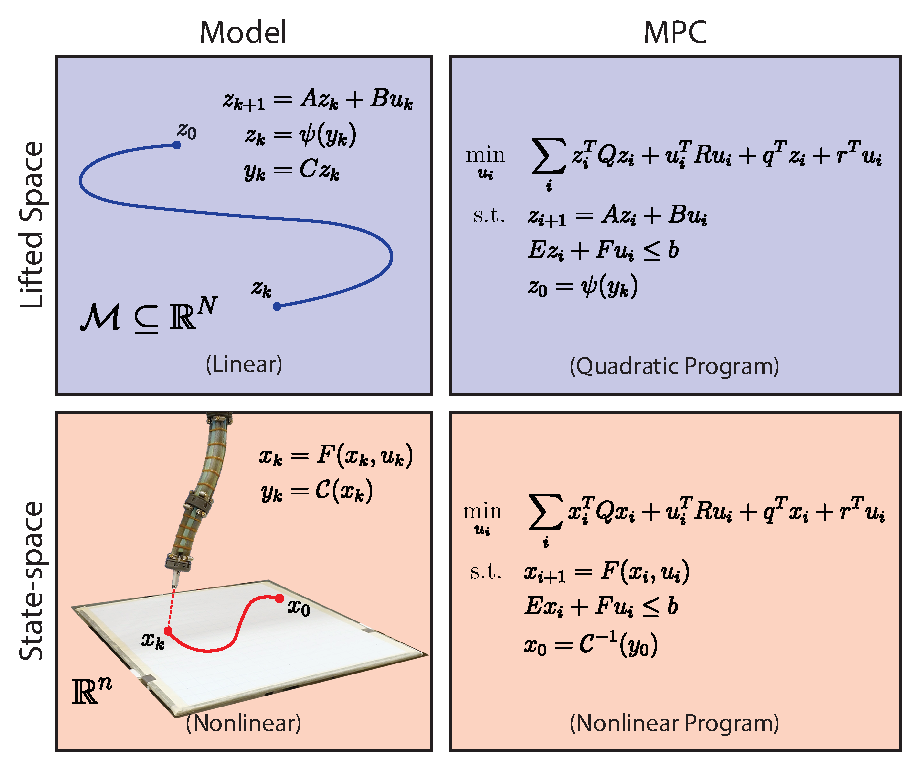
\includegraphics[width=\linewidth]{figures/overview_v7_ph.pdf}
    \caption{Caption}
    \label{fig:overview}
\end{figure}


%% Koopman approach exists and can help here, it just needs some tweaks to work well for a real system
Koopman Operator Theory offers an approach that can overcome the challenges of modeling and controlling nonlinear continuum systems.
Laid out in \citet{mauroy2016linear} and \citet{korda2018linear}, the approach leverages the linear structure of the Koopman operator to construct linear models for nonlinear controlled dynamical systems from input-output data, and control them using established linear control methods (such as model predictive control) \Ram{1. prolly want to cite our paper. 2. only the mezic paper does control. 3. probably want to cite the todd murphey paper.}.
In theory, this approach involves \emph{lifting} the state-space to an infinite-dimensional space of scalar functions (referred to as observables), where the flow of such observables along trajectories of the nonlinear dynamical system is described by the \emph{linear} Koopman operator.
In practice, however, it is not feasible to compute an infinite-dimensional operator, so a modified version of the Extended Dynamic Mode Decompostion (EDMD) is employed to compute a finite-dimensional projection of the Koopman operator onto a finite-dimensional subspace of all observables (scalar functions).
This approximation of the Koopman operator describes the evolution of the values of the output variables themselves, provided that they lie within the finite subspace of observables upon which the operator is projected.
Hence, this approach makes it possible to control the output of a nonlinear dynamical system using linear controllers designed for its linear Koopman representation \Ram{probably want to describe the shortcomings of this approach first?}.

%% Why this approach is uniquely well suited for soft robots: 
The Koopman approach to modeling and control is well suited for soft robots for several reasons.
Soft robots pose less of a physical threat to themselves or their surroundings when subjected to random control inputs than many conventional rigid bodied robots. 
This makes it possible to safely collect input-output data over a wide range of operating conditions, and to do so in an automated fashion. 
Furthermore, since the Koopman procedure is entirely data-driven, it inherently captures input-output behavior and avoids the ambiguity involved in choosing a discrete set of states for a continuum structure that has infinite degrees of freedom.
Soft robots are also nonlinear dynamical systems, but this approach generates a linear system representation.
As will be shown later, this linear representation can be used to construct a numerical controller which computes control inputs by solving a convex optimization problem at each time step.

%% Our contribution: Modifications/additions needed to get this to reliably work for a real system
\Ram{probably worth listing out all your contributions.}
In this work, we modify the Koopman system identification procedure of \citet{mauroy2016linear} and \citet{korda2018linear} to increase its efficacy when applied to real mechanical systems.
Specifically, we introduce an L1 penalty term into the least-squares optimization problem used to solve for the approximate Koopman operator.
This penalty term makes the result more robust to outliers in the training data, and promotes sparseness of the matrix representation of the operator.
Both of these are desirable features when working with real systems, which suffer from noise and computational limitations.

\Dan{Add comment about how real systems like ours have noise and need regularization (LASSO) to combat that in the model fit... (figure out best place to put it).}



%% Outline
The rest of this paper is organized as follows:
In Section \ref{sec:sysid} we formally introduce the Koopman operator and describe the procedure for constructing linear models of nonlinear systems. 
In Section \ref{sec:mpc} we describe how the Koopman model can be used to construct a linear model predictive controller for a nonlinear dynamical system.
In Section \ref{sec:experiments} we describe the soft robot used in our experiments and evaluate the performance of a Koopman-based MPC controller on a set of trajectory following tasks.
In Section \ref{sec:conclusion} concluding remarks and perspectives are provided.





% %% Solution: Data-driven/linear representation, description of koopman approach
% In this paper, we present a novel method for the modeling and control of soft robots based on Koopman Operator Theory.
% This method addresses the challenges of modeling and control by offering a way to build a \emph{linear} model from data that still captures the \emph{nonlinear} input-output behavior of a soft robot.
% This approach is based on the system identification method originally presented in \citet{mauroy2017koopman} and the control approach laid out in \citet{korda2018linear}.